 \documentclass{sig-alternate-05-2015}
\usepackage[linesnumbered,ruled]{algorithm2e}
\usepackage{color}
\usepackage{breqn}
\usepackage[export]{adjustbox}

\providecommand{\colorred}[1]{\textcolor{red}{#1}}

 
\begin{document}

\setcopyright{acmcopyright}

%\setcopyright{acmlicensed}
%\setcopyright{rightsretained}
%\setcopyright{usgov}
%\setcopyright{usgovmixed}
%\setcopyright{cagov}
%\setcopyright{cagovmixed}



\newtheorem{problem}{Problem}
\newtheorem{definition}{Definition}
\newtheorem{example}{Example}

\newcommand{\framework}{{\sc GeoHighlight}}
\newcommand{\pb}{{\sc GeoGuide}}

 
% DOI
\doi{10.475/123_4}

% ISBN
\isbn{123-4567-24-567/08/06}

%Conference
\conferenceinfo{PLDI '13}{June 16--19, 2013, Seattle, WA, USA}

\acmPrice{\$15.00}

\conferenceinfo{EDBT}{2016}

\title{GeoHighlight: A Point-Recommendation Approach for Spatiotemporal Data}
%\subtitle{[Extended Abstract]

\numberofauthors{3}


\author{
Behrooz Omidvar-Tehrani$^{\dag}$, Gustavo Guerino$^{\ddag \circ}$, Pl\'acido A. Souza Neto$^{\ddag \bullet}$\\
\affaddr{
$^{\dag}$The Ohio State University, USA, $^{\ddag}$Federal Institute of Rio Grande do Norte - IFRN, Brazil}\\
\affaddr{
$^{\dag}$\path{omidvar-tehrani.1@osu.edu},
$^{\circ}$\path{gustavo.guerino@academico.ifrn.edu.br},
$^{\bullet}$\path{placido.neto@ifrn.edu.br}
}}

% \date{30 July 1999}
% Just remember to make sure that the TOTAL number of authors
% is the number that will appear on the first page PLUS the
% number that will appear in the \additionalauthors section.

\maketitle
\begin{abstract}
Spatiotemporal data is becoming increasingly available in various domains such as transportation and social science. Discovering patterns and trends in this data provides improved insights for planning and decision making for smart city management, disaster management and other applications. However, exploratory analysis of such data is a challenge due to its huge size and diversity of spatiotemporal data. It is often unclear for the analyst {\em what to see next} during an analysis process, i.e., lack of guidance. To tackle this challenge, we formulate guidance as an optimization problem and develop \framework, an efficient interactive guidance approach for spatiotemporal data. At each step of an interactive process, $k$-most interesting geographical points become highlighted to guide the analyst through further steps. We illustrate the efficiency and usability of our framework in an extensive set of experiments.
\end{abstract}

% \keywords{Interactive analysis; Spatiotemporal visualization; Urban data.}

\vspace{-5pt}
\newpage
\section{Introduction}
Nowadays, there has been a meteoric rise in the generation of spatial datasets in various fields of science, such as transportation, lodging services and social science. As each record in spatial data represents an activity in a precise geographical location, analyzing such data enables discoveries grounded on facts. Analysts are often interested to observe spatial patterns and trends to improve their decision making process. Spatial data analysis has various applications such as smart city management, disaster management and autonomous transport \cite{RoddickEHPS04,Telang:2012}.

\vspace{2pt}
Typically, spatial data analysis begins with an imprecise question in the mind of the analyst, i.e., {\em exploratory analysis}. The analyst requires to go through several trail-and-error iterations to improve her understanding of the spatial data and gain insights. Each iteration involves visualizing a subset of data on geographical maps using an  off-the-shelf product (e.g., Tableau\footnote{\it http://www.tableau.com}, Exhibit\footnote{\it http://www.simile-widgets.org/exhibit/}, Spotfire\footnote{\it http://spotfire.tibco.com}) where the analyst can investigate on different parts of the visualization by zooming in/out and panning on the map. 

\vspace{3pt}
Spatial data are often voluminous. Hence the focus in the literature of spatial data analysis is on ``efficiency'', i.e., enabling fluid means of navigation in spatial data to facilitate the exploratory analysis. The common approach is to design pre-computed indexes which enable efficient retrieval of spatial data (e.g., \cite{lins2013nanocubes}). However, there has been fewer attention to the ``value'' derived from spatial data. Despite the huge progress on the efficiency front, an analyst may easily get lost in the plethora of geographical points due to two following reasons.

\vspace{3pt}
\noindent $\blacksquare$ In an exploratory context, the analyst doesn't know apriori what to investigate next.

\vspace{2pt}
\noindent $\blacksquare$ Moreover, she may easily get distracted and miss interesting points by visual clutter caused by huge point overlaps.

\vspace{3pt}
The main drawback of the traditional analysis model is that the analyst has a {\em passive role} in the process. In other words, the analyst's feedback (i.e., her likes and dislikes) is ignored and only the input query (i.e., her explicit request) is served. In case feedback is incorporated, the process can be more directed towards analyst's interests where her partial needs can be served earlier in the process. In this paper, we advocate for a ``guidance layer'' on top of the raw visualization of spatial data to enable analysts know {\em ``what to see next''}. This guidance should be a function of analyst feedback: the system should recommend options similar to what the analyst has already appreciated. 
% Hence, feedback capturing lies at the core of such guidance system.

\vspace{2pt}
Various approaches in the literature propose methodologies to incorporate analyst's feedback in the exploration process of spatial data. Typically, feedback is considered as a function which is triggered by any analyst's action on the map. The action can be ``selecting a point'', ``moving to a region'', ``asking for more details'', etc. The function then updates a ``profile vector'' which keeps tracks of analyst's interests. The updated content in the profile vector enables the guidance functionality. For instance, if the analyst shows interest in a point which describes a house with balcony, this choice of amenity will reflect her profile to prioritize other houses with balcony in future iterations.

\vspace{2pt}
Feedback is often expressed {\em explicitly}, i.e., the analyst clicks on a point and mentions if she likes or dislikes the point \cite{kamat2014distributed,Omidvar-Tehrani:2015,omidvar2017geoguide}. In \cite{omidvar2017geoguide}, we proposed an interactive approach to exploit such feedback for enabling a more insightful exploration of spatial data. However, there are several cases that the feedback is expressed {\em implicitly}, i.e., the analyst does not explicitly click on a point, but there exists correlations with other signals captured from the analyst which provide hint on her interest. For instance, it is often the case in spatial data analysis that analysts look at some regions of interest but do not provide an explicit feedback. Another example is frequent mouse moves around a region which is a good indicator of the analyst's potential interest in the points in that region. Implicit feedbacks are more challenging to capture and hence less investigated in the literature. The following example describes a use case of implicit feedbacks. This will be our running example which we follow thoughout the paper.

\vspace{2pt}
\noindent {\bf Example.} {\em Ben\'icio is planning to live in Paris for a season. He decides to rent a home-stay from Airbnb website\footnote{\it http://www.airbnb.com}. He likes to discover the city, hence he is open to any type of lodging in any region with an interest to stay in the center of Paris. The website returns 1500 different locations. As he has no other preferences, an exhaustive investigation needs scanning each location independently which is nearly infeasible. While he is scanning few first options, he shows interest in the region of Trocadero (where the Eiffel tower is located in) but he forgets or doesn't feel necessary to click a point there. An ideal system should capture this implicit feedback in order to short-list a small subset of locations that Ben\'icio should consider as high priority}.

\vspace{2pt}
The above example shows in practice that implicit feedback capturing is crucial in the context of spatial data analysis. While text-boxes, combo-boxes and other input elements are available in analyzing other types of data, the only interaction means between the analyst and a spatial data analysis system is a geographical map spanned on the whole screen. In this context, a point can be easily remained out of sight and missed.

\vspace{2pt}
In this paper, we present an approach called {\sc GeoPoly} whose aim is to capture and analyze implicit feedback of analysts in spatial data analysis. Without loss of generality, we focus on ``mouse moves'' as the implicit feedback received from the analyst. Mouse moves are the most common way that analysts interact with geographical maps~\cite{Chen:2001}. It is shown in \cite{Arapakis:2014} that mouse gestures have a strong correlation with ``user engagement''. Intuitively, a point gets a higher weight in the analyst's profile if the mouse cursor moves around it frequently.  However, our approach can be easily extended to other types of inputs such gaze tracking, leap motions, etc.

% \cite{Robertson2007}  affirms that temporal change in spatial patterns are increasingly common in geographical analysis. This work explore an approach to the spatialtemporal analysis of polygons that are spatially distinct and experience discrete changes though time. It presents challenges considering changes of regions (polygons) during the time. Works like \cite{Ester:1996} and  \cite{Birant:2007} present solutions for clustering spatialtemporal data. These solutions are relevant to define regions by each cluster that contains important informations for the user. 

% \vspace{3pt}
% Discovering patterns and provide tendencies in spatial data applications may improve insights for planning and decision making for smart city solutions. Many systems and datasets consider space information.  In this way, find spatial preferences can offer interactive and guidance solutions.  For example,  when users look for a house or hotel to spend a season, they consider one or more regions of their preference. These regions are intrinsic to each user, or user group. However, when navigating the application, the user also considers regions that seem interesting, for different reasons, such as the priority of some tourist spot, restaurants, clubs, security, etc. Thus, capturing region preferences over time can help to guide the user to find better places.
 
% \vspace{3pt}
% Given a dataset of spatial points and from the mouse tracking movements by the user, our approach generates a set of highlighted regions based on its preferences. Each region is related with a subset of highlighted points which are illustrated using visual variables such as size and color intensity. The regions are also highlighted.

\vspace{2pt}
The outline of the paper is the following. Section \ref{sec:datamodel} describes our data model. In Section \ref{sec:problem}, we formally define our problem. Then in Section \ref{sec:algo}, we present our solution and its algorithmic details. Section  \ref{sec:exp} reports our experiments on the framework. We review the related work in Section \ref{sec:rel}. Last, we conclude in Section \ref{sec:conc}.
% \section{Data Model}\label{sec:data-model}
% prune this
% A wide range of spatiotemporal data is present in a vast variety of datasets such as aviation, ground transportation (bike, taxi, renting- car, bus), urban data, geo-tagged social networks, crimes, events, etc. Intuitively, the common point between all those dataset is having {\em location} and {\em time} attributes. Based on this particularity, we propose a generic data model to capture all diverse aspects of such data.

We consider a spatiotemporal database ${\cal D}$ consisting $\langle {\cal P}, {\cal A} \rangle$ where ${\cal P}$ is the set of
geographical points and ${\cal A}$ is the set of point attributes. For each $p \in {\cal P}$, we consider a tuple $\langle lat, lon, alt, t\rangle$ where $lat$, $lon$ and $alt$ denote $p$'s geographical coordinates (latitude, longitude and altitude respectively), and $t$ is the timestamp. The set ${\cal A}_p$ contains attribute-values for $p$ over the schema of ${\cal A}$. For instance, on a bike-sharing dataset, ${\cal A}_p = \langle${\tt female}, {\tt young}, {\tt hybrid-bike}$\rangle$ on the schema ${\cal A} = \langle${\tt gender}, {\tt age}, {\tt type}$\rangle$ denotes that $p$ is associated to a young female cyclist who rides a hybrid bike. The set ${\cal A}$ is domain-dependent and defines the semantics of a spatiotemporal dataset. 
% For instance, in case of a taxi dataset, ${\cal A} = \langle$ {\tt dropoff\_time}, {\tt price}, {\tt tip} $\rangle$, where for an aviation dataset, ${\cal A} = \langle$ {\tt aircraft\_type}, {\tt departure\_airport}, {\tt arrival\_airport} $\rangle$.

% prune this
% Some spatiotemporal datasets contain point-sets as entities, such as {\em trajectories} in transportation datasets and {\em regions} in urban or agriculture dataset. Although our generic data model only captures the finest granular concept (i.e., point), we define ${\cal S}$ containing point-sets. Each point-set $s \in {\cal S}$ is indeed a set of points where $s \subseteq {\cal P}$. For instance, in a taxi dataset, $s = [ p_1, p_2 \dots p_n ]$ shows a ride consisting $n$ points departing at $p_1$ and arriving at $p_n$.
\vspace{-5pt}
\section{Problem Statement}
\label{sec:pb}
% In an exploratory analysis context, the analyst does not necessarily know what to ask. She may have also a few knowledge about the spatiotemporal data and its attributes. Hence she usually needs to take iterative analysis steps to observe different aspects of data and ultimately land on a subset of interest. However, it is often cumbersome to choose what to analyze next. Because this choice is subjective and infeasible to capture with an unsupervised method.

\noindent {\bf Data Model.} We consider a spatiotemporal database ${\cal D}$ consisting $\langle {\cal P}, {\cal A} \rangle$ where ${\cal P}$ is the set of
geographical points and ${\cal A}$ is the set of point attributes. For each $p \in {\cal P}$, we consider a tuple $\langle lat, lon, alt, t\rangle$ where $lat$, $lon$ and $alt$ denote $p$'s geographical coordinates (latitude, longitude and altitude respectively), and $t$ is the timestamp. The set ${\cal A}_p$ contains attribute-values for $p$ over the schema of ${\cal A}$. For instance, on a bike-sharing dataset, ${\cal A}_p = \langle${\tt female}, {\tt young}, {\tt hybrid-bike}$\rangle$ on the schema ${\cal A} = \langle${\tt gender}, {\tt age}, {\tt type}$\rangle$ denotes that $p$ is associated to a young female cyclist who rides a hybrid bike. The set ${\cal A}$ is domain-dependent and defines the semantics of a spatiotemporal dataset.

\vspace{5pt}
In this paper, we address the problem of {\em generic guidance} in spatiotemporal data: ``what is the process of guiding analysts in iterative analysis steps on any spatiotemporal dataset?'' In other words, we are interested in an approach which highlights a set of $k$ points that the analyst should consider in the next analysis iteration. This should not be a heuristic-based data-dependent highlighting, but a generic approach which is applied on any spatiotemporal dataset. We describe the desiderata of generic guidance approach as follows.

\vspace{5pt}
\noindent {\bf D1. Genericness.} The guidance component should be agnostic (making no assumption) about the dataset type, attributes and distribution. In other words, the guidance approach should not be a function of any property of data.

\vspace{5pt}
\noindent {\bf D2. Limited Options.} The set of $k$ highlighted points should not be very large because too many options distract the analyst. % \cite{miller1956human}.

\vspace{5pt}
\noindent {\bf D3. Relevance.} The fundamental difference between highlighting and $k$-NN spatial queries \cite{aly2015spatial} is that, in the former, the focus is on $k$ points which have similar characteristics to~$p$, hence relevant.
% In other words, we are interested in points which are {\em relevant} to a given point of interest.
For instance, consider a taxi ride in New York for a young male customer for an itinerary of 10 kilometers and \$3 tip. In contrary to thousands of kilometers of geographical distance, the ride is very similar to another one in San Fransisco for a middle-age male customer for an itinerary of 8 kilometers and \$2.5 tip.
% Relevance is a pairwise metric which is associated to point characteristics.
Given two points $p$ and $p'$, we define {\em relevance} as follows.

% \begin{definition}[Relevance]
% Given two points $p$ and $p'$ and their attribute values ${\cal A}_{p}$ and ${\cal A}_{p'}$, the relevance between $p$ and $p'$ is a value between $0$ and $1$ denoted as $\mathit{relevance}(p,p') = \mathit{average}_{a \in {\cal A}_{p} \cup {\cal A}_{p'}}(\mathit{sim({\cal A}_{p}, {\cal A}_{p'}, a)})$.
% \label{def:rel}
% \end{definition}

\begin{dmath}
\label{eq:rel}
\mathit{relevance}(p,p') = \mathit{average}_{a \in {\cal A}_{p} \cup {\cal A}_{p'}}(\mathit{sim(p, p', a)})
\end{dmath}

The similarity function $\mathit{sim}()$ can be any function such as Jaccard and Cosine. Each attribute can have its own similarity function (as string and integer attributes are compared differently.) Then $\mathit{sim}()$ works as an overriding-function which provides encapsulated similarity computations for any type of attribute.

\vspace{5pt}
\noindent {\bf D4. Diversity.} A guidance approach should also consider coverage of all points: $k$ highlighted points should represent distinct regions so that the analyst can observe different aspects of data and decide for the next analysis iteration. Hence, $k$ points should be diverse.
% Diversity is a set-based metric and is associated to geographical distance. We define this metric as follows.
Given a set of points $s = \{ p_1, p_2 \dots \}$, we define {\em diversity} as follows.

\begin{dmath}
\label{eq:divs}
\mathit{diversity}(s) = \mathit{average}_{\{p, p'\} \subseteq s | p \neq p' } \mathit{distance}(p,p')
\end{dmath} 

The function $\mathit{distance}(p,p')$ operates on geographical coordinates of $p$ and $p'$ and can be considered as any distance function of Chebyshev distance family such as Eucledian. However, as distance computations are done in {\em spherical space} using latitude, longitude and altitude, it is au-naturel to employ Harvestine distance shown in Equation \ref{eq:harvestine}.

\begin{dmath}
\label{eq:harvestine}
distance(p,p') = [ acos(cos(p_{lat}) . cos(p'_{lat}) . cos(p_{lon}) . cos(p'_{lon})\\ + cos(p_{lat}) . sin(p'_{lat}). cos(p_{lon}) . sin(p'_{lon}) + sin(p_{lat}) . sin(p'_{lat})) ] \times earth\_radius
\end{dmath}

\noindent {\bf D5. Interactivity.} The exploratory nature of the analysis requires the guidance component to be involved in an interactive process. Hence the analyst can investigate and refine different aspects of spatiotemporal data in iterative steps. For being interactive, the guidance component should be efficient so that the train of thought of analyst would not be broken during the analysis process.

\vspace{5pt}
Following aforementioned desiderata, we formulate highlighting as an optimization-based problem on relevance and diversity dimensions.

\begin{problem}[\pb]
\label{pb:geoh}
Given an input point $p$ and a threshold $\sigma$, the problem is to return top-$k$
 points denoted $S_p$ where $|S_p| = k$ and $\forall p' \in S_p, \mathit{relevance}(p,p') \geq \sigma$ and $\mathit{diversity}(S_p)$ is maximized.
\end{problem}

Problem \ref{pb:geoh} is hard due to the huge space of spatiotemporal data: for any given point $p$, an exhaustive search over all other points is necessary to find $k$ points with maximal relevance. Moreover, the problem investigates in two dimensions at the same time (relevance and diversity) which makes it more challenging.

% behrooz: talk about quality earlier

\vspace{-5pt}
\section{Algorithm}
\label{sec:algo}
We propose a solution for \pb\ by inspiring from both recommendation \cite{Omidvar-Tehrani:2015} and
visual highlighting
% \cite{Lohmann:2012,Robinson2011,Liang2010}
\cite{Liang2010,Robinson2011}
methodologies. \pb\ requires an efficient algorithm for dynamically analyzing and comparing geographical points. We propose \framework\ as a solution for the generic guidance problem in spatiotemporal data (Figure \ref{fig:framework}). Although \framework\ operates on points, its functionality can be easily extended to regions using point-clustering methods such as $k$-means.

\framework\ operates in two steps: {\sc Preparation} and {\sc Highlighter}. In order to speed up computing relevance in online execution, we pre-compute an inverted index for each single geographical point in ${\cal P}$ in the offline {\sc Preparation} step (as is commonly done in Web search). Each index ${\cal L}_p$ for the point $p$ stores all other points in ${\cal P}$ in decreasing order of their relevance with $p$. Thanks to the parameter $\sigma$, we only partially materialize the indexes.

% behrooz: explain the whole package

Algorithm \ref{algo:geoh} illustrates the online execution step of \framework\, so called {\sc Highlighter}. The algorithm is a single greedy procedure that solves the \pb\ problem. {\sc Highlighter} is called at each interactive step of \framework\ (as in Figure \ref{fig:framework}). The algorithm admits as input a point $p \in {\cal P}$ and returns the best $k$ points denoted ${\cal S}_p$.

To comply with the desiderata {\bf D5}, we consider a time limit parameter $tlimit$ in Algorithm \ref{algo:geoh}. In a {\em best-effort} strategy, the algorithm bounds user waiting time by $tlimit$ to return the best possible results by then.

\begin{algorithm}[t]
\DontPrintSemicolon
\KwIn{$p \in {\cal P}$, $\sigma$, $k$, $tlimit$}
% \KwOut{${\cal S}_p$}
${\cal S}_p \gets get\_top\_k(\mathit{{\cal L}^p})$\;\label{cd:gettopk}
$p_{next} \gets get\_next(\mathit{{\cal L}^p})$\;\label{cd:getnext}
\While{$(tlimit$ $not$ $exceeded \wedge relevance(p,p_{next}) \geq \sigma)$}{\label{cd:beginwhile}
\For{$p_{current} \in {\cal S}_p$}{
\If{$\mathit{diversity\_improved}({\cal S}_p,p_{next},p_{current})$}{\label{cd:betterdiv}
${\cal S}_p \gets \mathit{replace}({\cal S}_p,p_{next},p_{current})$\;
$break$\;
}
}
$p_{next} \gets get\_next({\cal L}^p)$\;}\label{cd:endwhile}
\Return{${\cal S}_p$}\; 
\caption{{\sc Highlighter} Algorithm}
\label{algo:geoh}
\end{algorithm}
% \vspace{-10pt}
% behrooz: mention working of sacrification

{\sc Highlighter} begins by retrieving the most relevant points to $p$ by simply retrieving the $k$ highest ranking points in ${\cal L}_p$ (line \ref{cd:gettopk}). Function $get\_next({\cal L}_p)$ (Line \ref{cd:getnext}) returns the next point $p_{next}$ in ${\cal L}_p$ in sequential order. Lines \ref{cd:beginwhile} to \ref{cd:endwhile} iterate over the inverted indexes to determine if other points should be considered to increase diversity while staying within the time limit and not violating the relevance threshold with the selected point. Since points in ${\cal L}_g$ are sorted on decreasing relevance with $p$, the algorithm can safely stop as soon as the relevance condition is violated (or if the time limit is exceeded).

The algorithm then looks for a candidate point $p_{current} \in {\cal S}_p$ to replace in order to increase diversity. The boolean function $\mathit{diversity\_improved}()$ (line \ref{cd:betterdiv}) checks if by replacing $p_{current}$ by $p_{next}$ in ${\cal S}_p$, the overall diversity of the new ${\cal S}_p$ increases.

% \vspace{5pt}
% \noindent {\bf Complexity Analysis.} The number of diversity improvement loops (lines \ref{cd:beginwhile} to \ref{cd:endwhile}) is $|{\cal L}_p| = |{\cal P}|$ in worst case. For each point $g_{current} \in {\cal S}_p$, we verify if the diversity score is improved by $\mathit{diversity\_improved}()$, hence $\mathcal{O}(k^2$). The time complexity of the algorithm is then $\mathcal{O}(k^2.|{\cal P}|)$.

\vspace{-5pt}
\section{Illustrative Scenario}\label{sec:scenarios}
We illustrate an application of \framework\ in a realistic scenario for New York taxi dataset\footnote{\it https://data.cityofnewyork.us/view/gn7m-em8n}. This dataset has been frequently exploited for urban analysis
% \cite{ferreira2013visual,DBLP:journals/debu/FreireCVZ16}.
(e.g. in \cite{DBLP:journals/debu/FreireCVZ16}).
The dataset contains 173,179,759 records of taxi trips and 18 attributes such as pickup and dropoff date/time, passenger count and trip distance.
% The dataset size is 27.9 GB with informations of trips from 2014.
The scenario illustrates how an analyst can achieve an exploratory analysis goal. We preprocessed the original dataset and considered a subset of 20K unique points for the sake of clarity of results. We employ {\sc Highlighter} (Algorithm \ref{algo:geoh}) with following parameters: $\sigma = 0.2$, $k = 5$ and $tlimit = 200ms$.

\begin{figure}
  \centering
  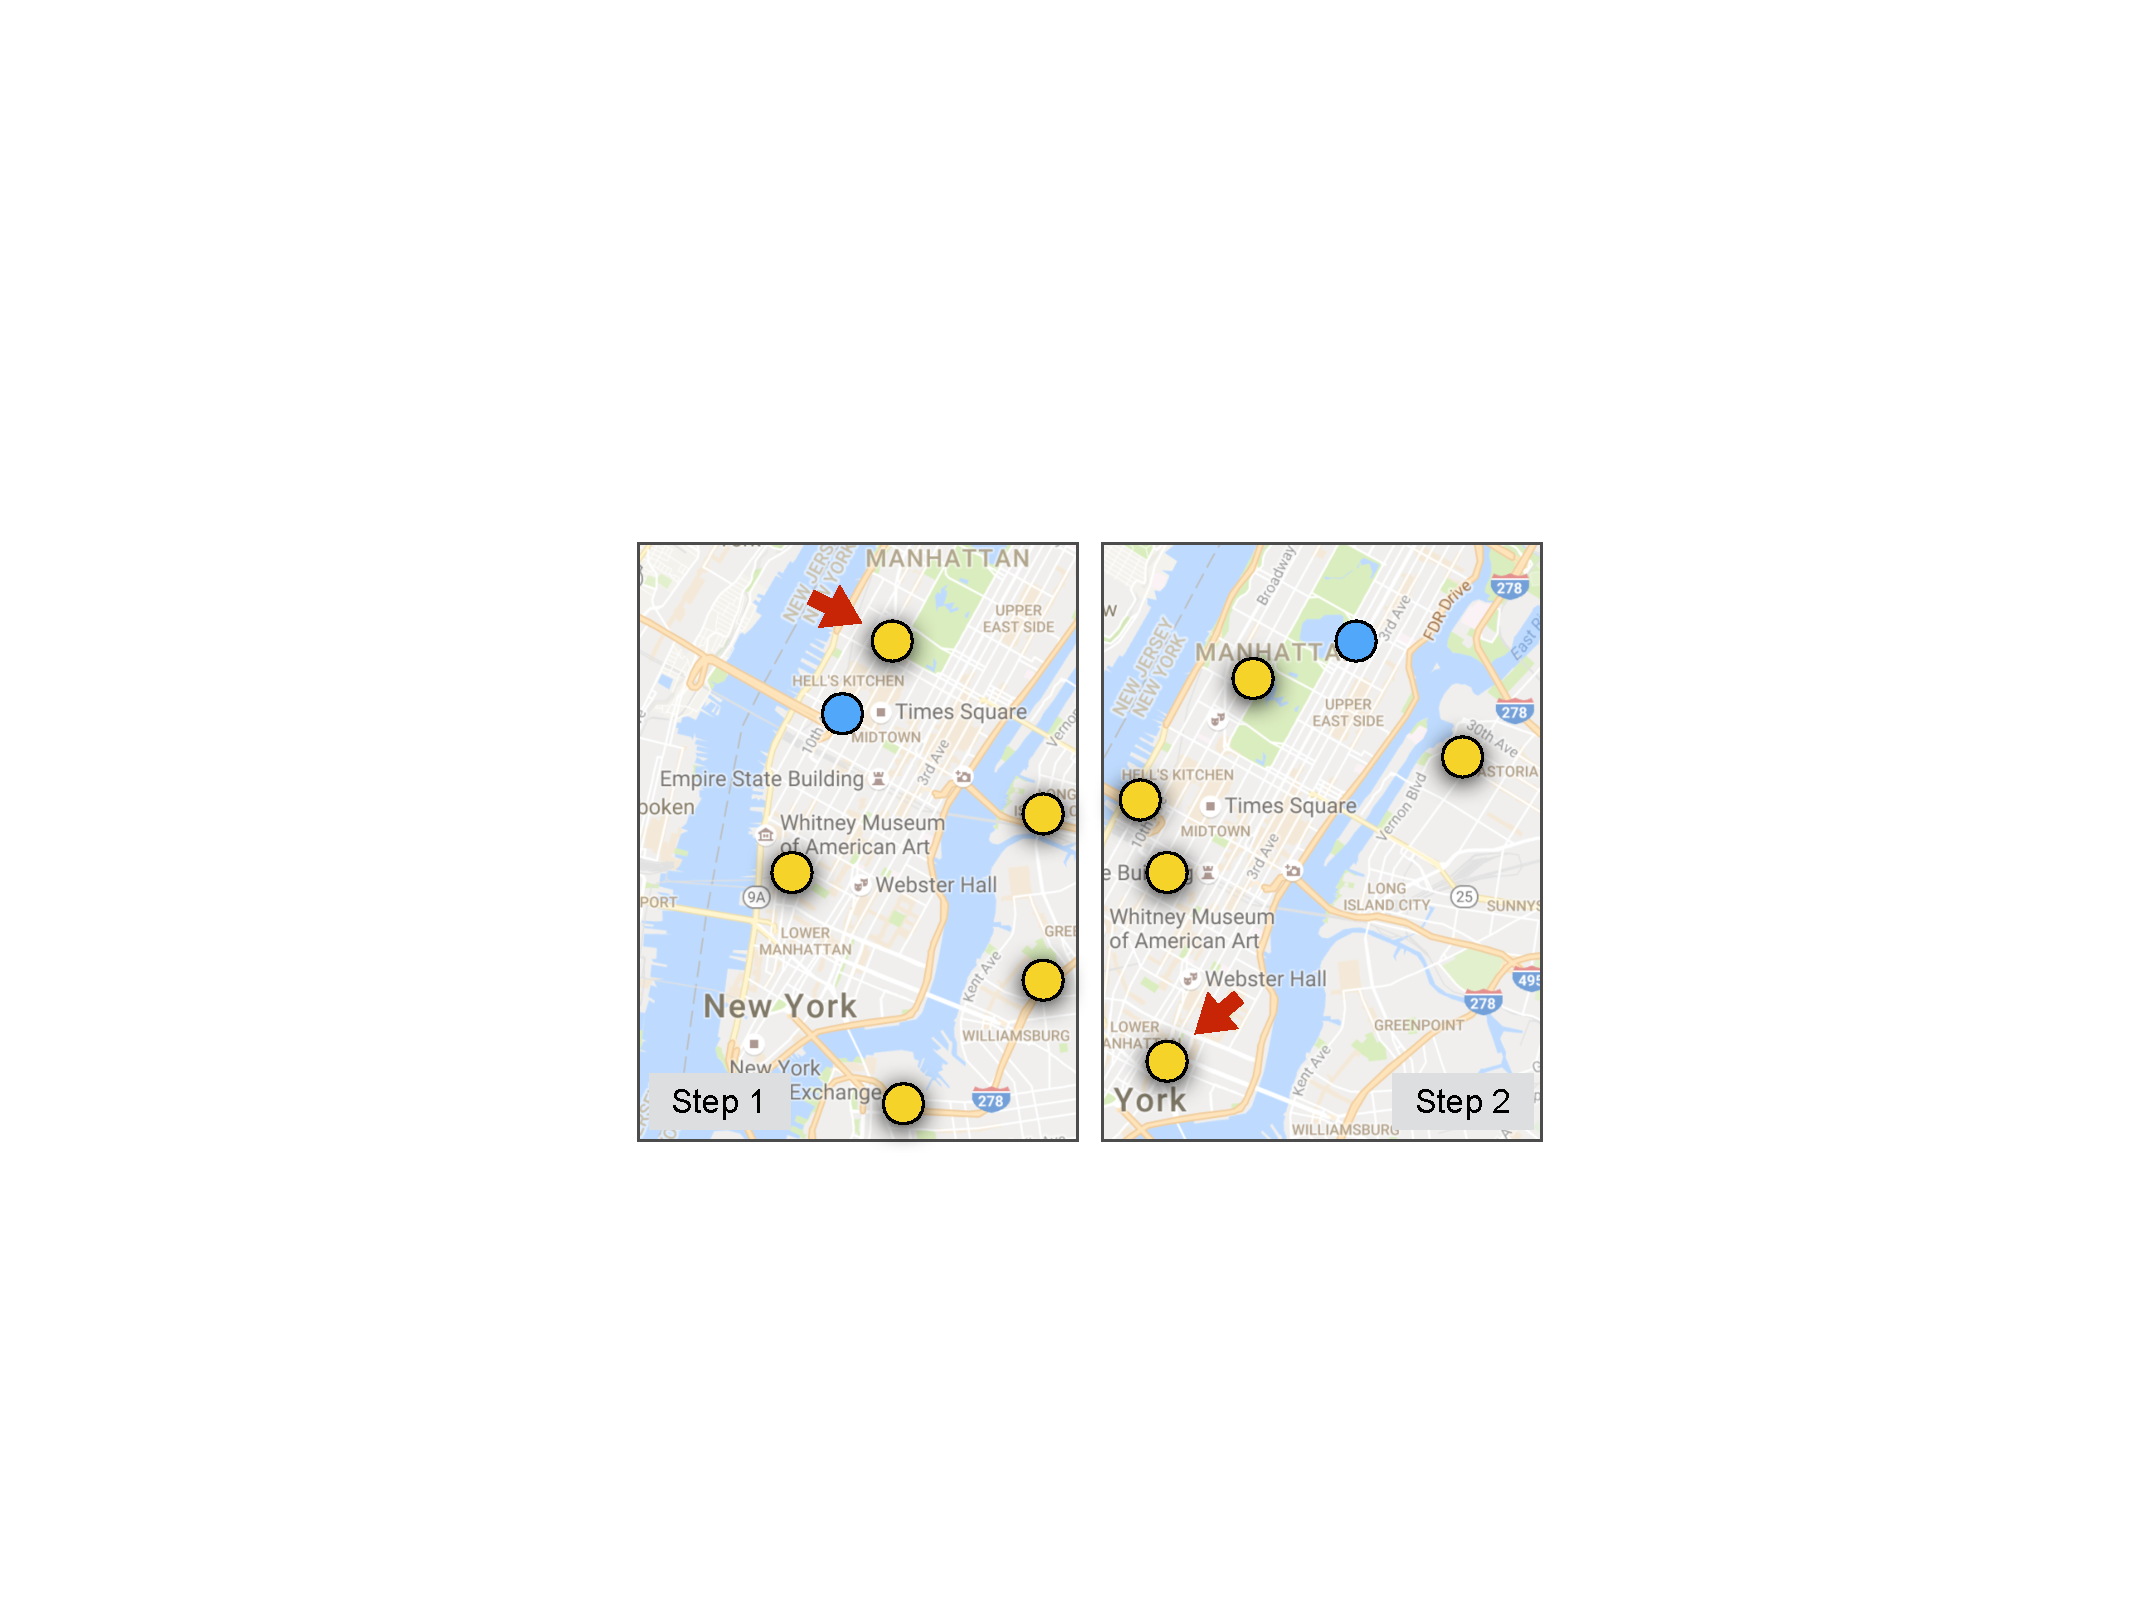
\includegraphics[width=\columnwidth]{figs/scn}
\caption{Application of \framework}
\label{fig:app}
\vspace{-10pt}
\end{figure}


% \vspace{5pt}
Consider Lucas, a data scientist whose task is to optimize New York taxi trips. Focusing on cab-idle locations, he wants to discover which neighborhoods work the best for which drivers to increase the overall availability. Also, he wants to discover how drivers should choose their next cab-idle station to be more available. Lucas employs \framework\ and follows a case-by-case inspection as his analysis methodology by analyzing and learning from historical data.

% coordinates of first point picked: lat, long: 40.757555, -73.988832. Point ID-1274, equivalent to 270 W 43rd St, New York, NY 10036, EUA. Next to Times Square.
% coordinates of the second point: lat, long: 40.789358,-73.970172000000005. Point ID-968, equivalent to Columbus Avenue, New York, NY, EUA.
%  coordinates of the third point: lat, long: 40.717531999999999,-74.010260000000002. Point ID-192, equivalent to 183 Duane Street, New York, NY 10013, EUA

He begins the analysis by selecting a point from the most crowded region in New York, i.e., Times Square (Figure \ref{fig:app} left). The point depicts a drop-off at {\em ``3 Times Square, New York, NY''} on January 9, 2014 around 9PM (the blue point in the figure). {\sc Highlighter} then provides $5$ relevant points to the selected point (yellow points in the figure).
% These highlights show similar points to the selection in other neighborhoods of the region.
Among 5 highlighted points, Lucas selects a pick-up at {\em ``West 53rd Street''} near Central Park occurred approximately at the same time of the first selection (the point marked with an arrow in the figure). This pick-up has a potential to enchain with the first choice (i.e., a drop-off) to engage the driver in a larger distance.

In the next step, {\sc Highlighter} shows $5$ other points relevant to the new selection (Figure \ref{fig:app} right). Lucas looks for a good drop-off point which is in a neighborhood of the previous selection as the cab-idle station. Lucas selects a highlight in downtown as others are around the train station which have often less taxi requests at nights. This selection contributes to the heavy cab request in Manhattan island at that time of the day. Note that in both steps, the $k$ results are a compromise between relevance and diversity.

% The result of similarity for all two executions of the algorithm for the Lucas problem, considering $k = 5$ and $\sigma = 0.2$, was approximately, \textit{0.72}.

\vspace{-5pt}
\section{Experiments}
\label{sec:exp}
We evaluate the efficiency and usefulness of \framework\ in an extensive set of experiments. We consider two types of experiments: first, a performance study measures the influence of relevance and size constraint thresholds on execution time. Second, we measure the usefulness of our framework in a user study.

\vspace{5pt}
\noindent {\bf Experiment Settings.} Unless otherwise stated, we use the same settings discussed in Section \ref{sec:scenarios}. All experiments are implemented in Python (functionality) and JavaScript D3 (visualization) on a 2.8GHz Intel Core i5 machine with an 16GB main memory, running OS X 10.9.2.

\begin{figure}
 \centering
 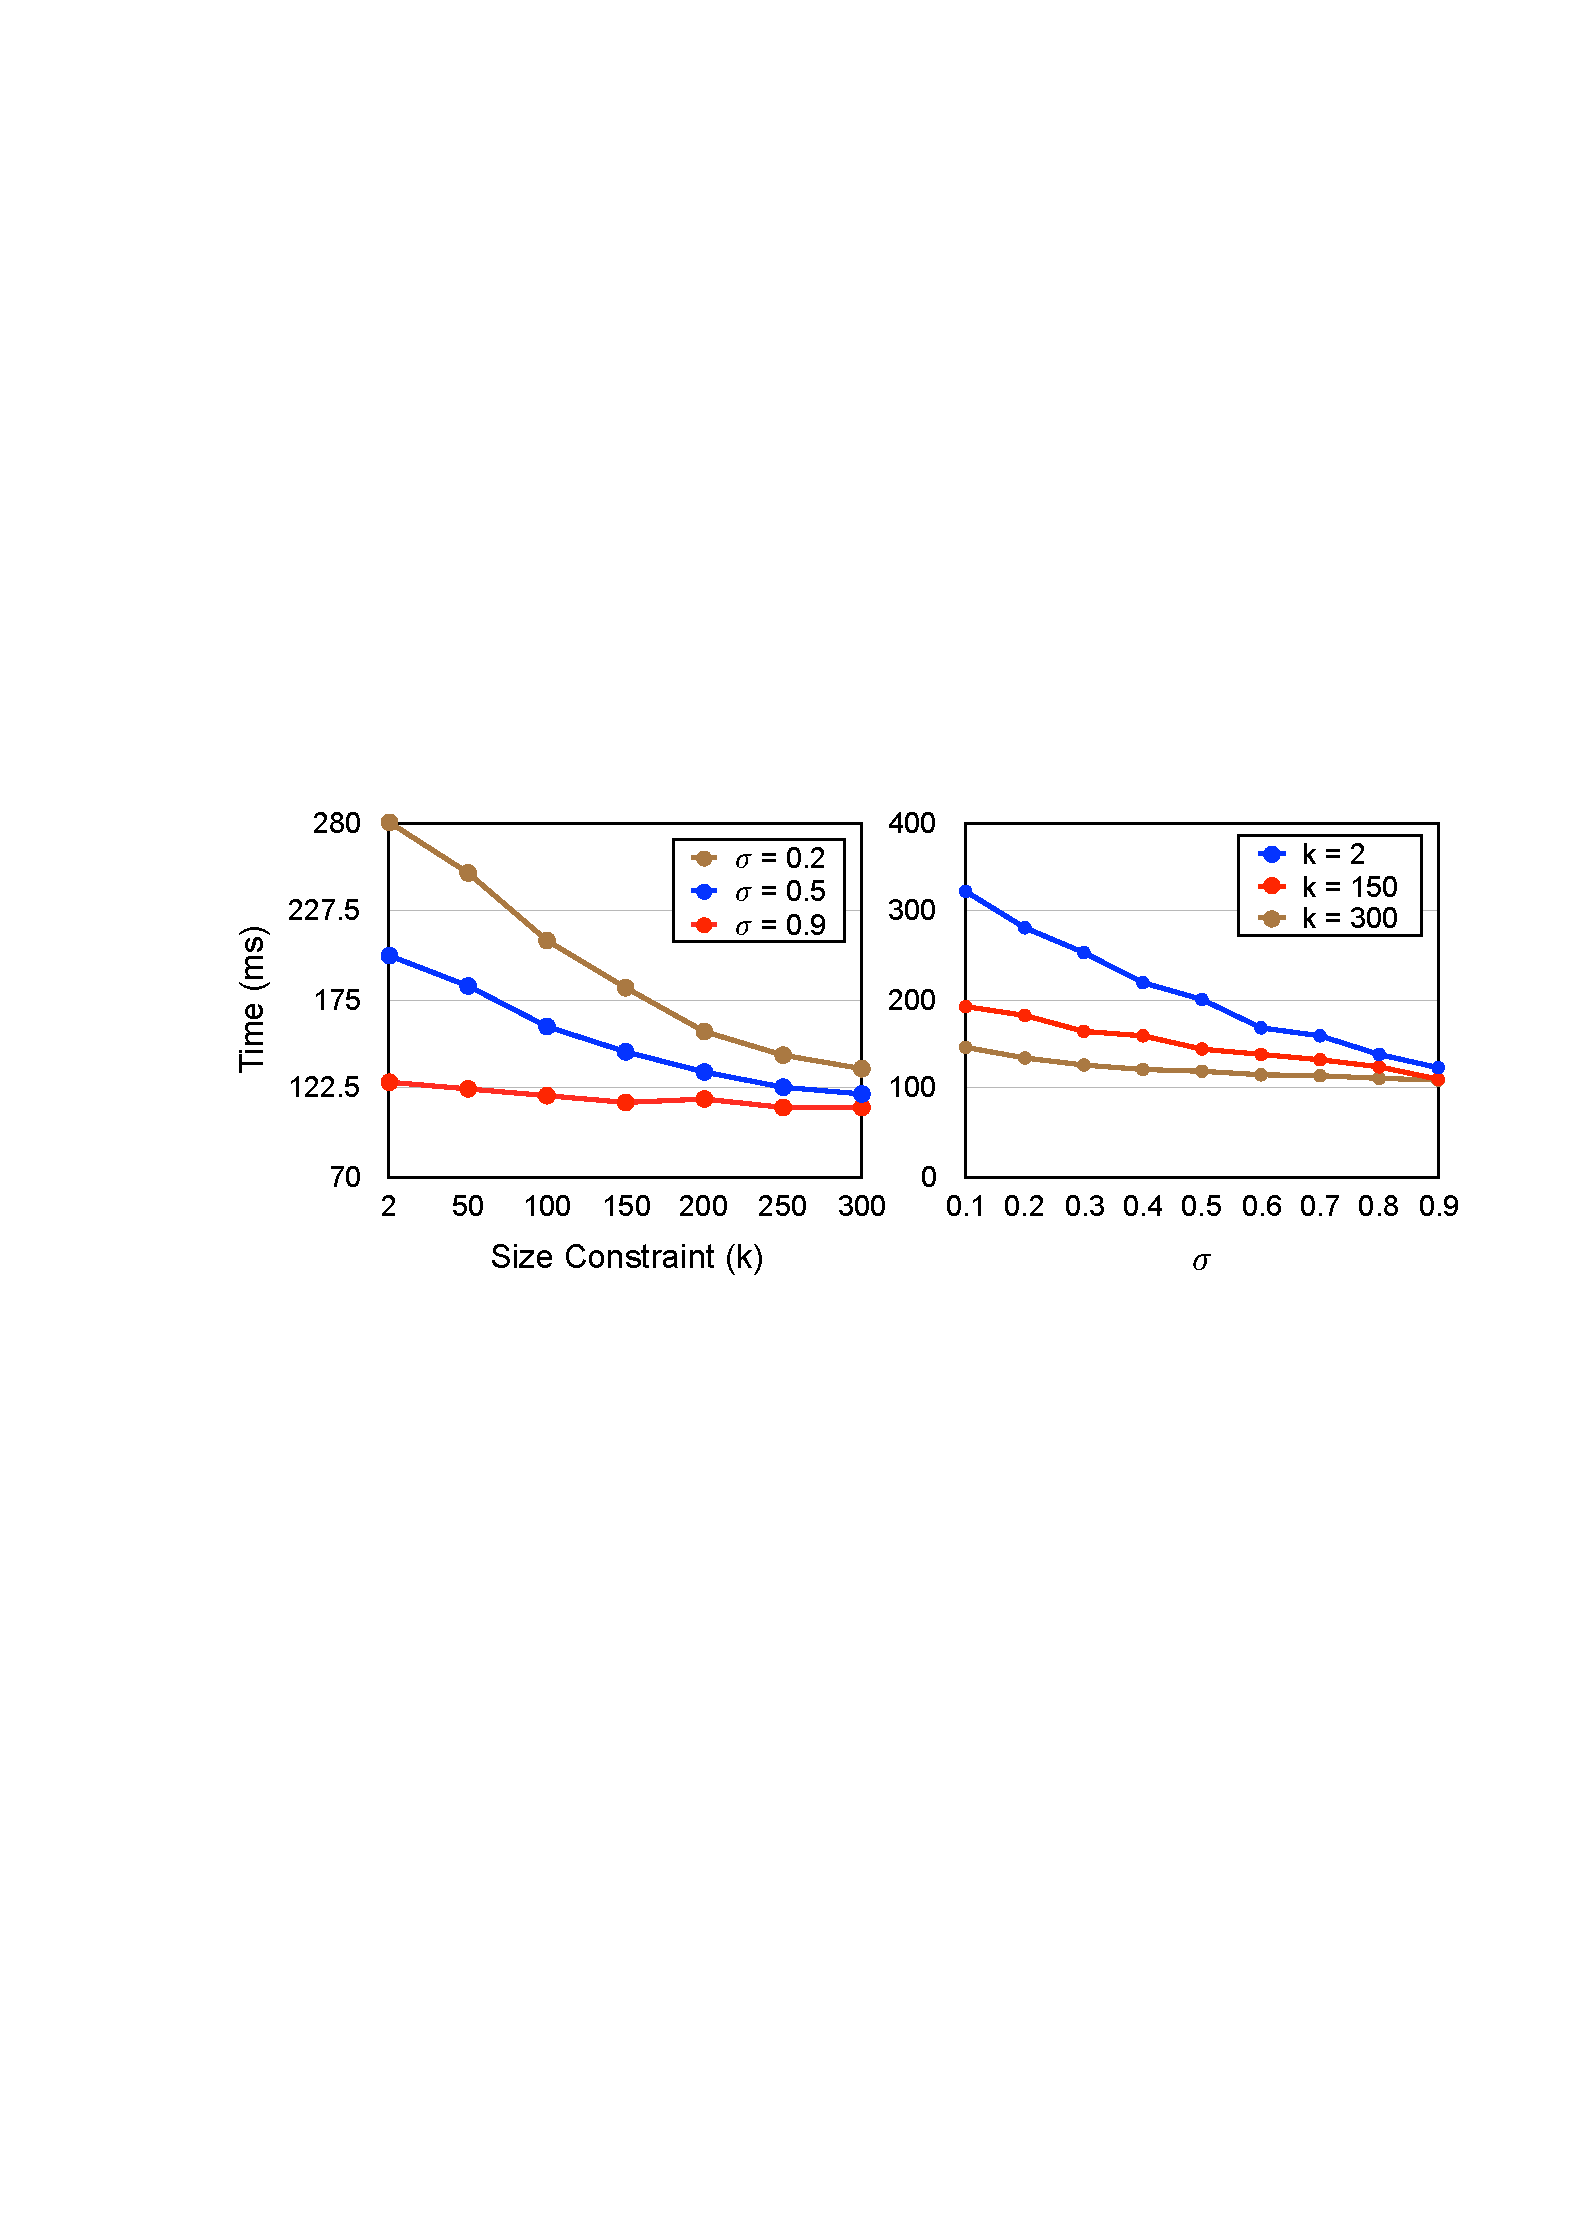
\includegraphics[width=\columnwidth]{figs/performance}
\caption{Performance Evaluation}
\vspace{-10pt}
\label{fig:performance}
\end{figure}

% \begin{figure}
%   \centering

% % Preamble: 
% \pgfplotsset{width=\columnwidth,compat=1.13}
% \tiny
% \begin{minipage}[b]{0.45\linewidth}
% \begin{tikzpicture}
% \begin{axis}[
% 	xlabel={Size Constraint (k)},
% 	ylabel={Similarity}
% ]

% \addplot table [x=k, y=sim, col sep=comma] {figs/charts/c01/02.csv};
% \addplot table [x=k, y=sim, col sep=comma] {figs/charts/c01/05.csv};
% \addplot table [x=k, y=sim, col sep=comma] {figs/charts/c01/07.csv};
% \addplot table [x=k, y=sim, col sep=comma] {figs/charts/c01/09.csv};

% \tiny
% %\legend{$\sigma=0.2$, $\sigma=0.5$, $\sigma=0.9$}
% \end{axis}
% \end{tikzpicture}
% \end{minipage}
% \hspace{0.2cm}
% \begin{minipage}[b]{0.45\linewidth}
% \begin{tikzpicture}
% \begin{axis}[
% 	xlabel={Size Constraint (k)},
% 	ylabel={Diversity}
% ]

% \addplot table [x=k, y=div, col sep=comma] {figs/charts/c01/02.csv};
% \addplot table [x=k, y=div, col sep=comma] {figs/charts/c01/05.csv};
% \addplot table [x=k, y=div, col sep=comma] {figs/charts/c01/07.csv};
% \addplot table [x=k, y=div, col sep=comma] {figs/charts/c01/09.csv};
% \tiny
% %\legend{$\sigma=0.2$, $\sigma=0.5$, $\sigma=0.9$}
% \end{axis}
% \end{tikzpicture}
% \end{minipage}

% %%% SECOND LINE %%% 
% \bigskip

% \begin{minipage}[b]{0.45\linewidth}
% \begin{tikzpicture}
% \begin{axis}[
% 	%legend pos=outer north east,
% 	xlabel={Size Constraint (k)},
% 	ylabel={Time(sec)}
% ]

% \addplot table [x=k, y=0.2, col sep=comma] {figs/charts/fig3.csv};
% \addplot table [x=k, y=0.5, col sep=comma] {figs/charts/fig3.csv};
% \addplot table [x=k, y=0.7, col sep=comma] {figs/charts/fig3.csv};
% \addplot table [x=k, y=0.9, col sep=comma] {figs/charts/fig3.csv};
% \tiny
% %\legend{$\sigma=0.2$,$\sigma=0.5$,$\sigma=0.7$,$\sigma=0.9$}
% \end{axis}
% \end{tikzpicture}
% \end{minipage}
% \hspace{0.2cm}
% \begin{minipage}[b]{0.45\linewidth}
% \begin{tikzpicture}
% \begin{axis}[
% 	%legend pos=outer north east,
% 	xlabel={Sigma ($\sigma$)},
% 	ylabel={Time(sec)}
% ]

% \addplot table [x=sigma, y=2, col sep=comma] {figs/charts/fig4.csv};
% \addplot table [x=sigma, y=100, col sep=comma] {figs/charts/fig4.csv};
% \addplot table [x=sigma, y=200, col sep=comma] {figs/charts/fig4.csv};
% \addplot table [x=sigma, y=300, col sep=comma] {figs/charts/fig4.csv};

% \tiny
% %\legend{$k=2$,$k=100$,$k=300$,$k=300$}
% \end{axis}
% \end{tikzpicture}
% \end{minipage} 
%   \caption{Performance Evaluation}
% \vspace{-10pt}
% \label{fig:performance}
% \end{figure}

\newpage
% \vspace{-20pt}
\noindent {\bf Performance Study.} \framework\ is designed for exploratory context where interactivity is a need. The ``best-effort'' greedy approach of {\sc Highlighter} (Algorithm \ref{algo:geoh}) guarantees to return the best possible results within a time limit. We consider a large time limit ($tlimit = 2s$) in order to evaluate the effect of relevance and size constraint thresholds on execution time.
% Figure \ref{fig:performance} illustrates the results by measuring the execution time.

Figure \ref{fig:performance} left illustrates the effect of size constraint by varying $k$ from $2$ to $300$. In general, larger values of $\sigma$ provides more freedom for the algorithm hence more time-consuming. An interesting observation is that increasing $k$ leads decreasing execution time. This is because in larger sets, there exist fewer opportunities for increasing diversity, hence {\sc Highlighter} terminates early.

Figure \ref{fig:performance} right confirms that lower values of $\sigma$ decreases execution time as they provide more flexibility for diversity improvement. For larger values of $k$ (i.e., when $k >100$), the influence of $\sigma$ on execution time becomes insignificant.

\vspace{5pt}
\noindent {\bf User Study.}
The principled question that we ask ourselves is whether \framework\ is useful for analysts in practice. To answer this question, we designed a user study with $24$ participants (students in Computer Science). Half of the participants know the New York region well (experts) and the other half have a limited knowledge (novice). In our user study, we define a task for each participant and ask him/her to fulfill the task using both \framework\ and {\sc Tableau} (as the most advanced spatiotemporal visualization tool). Then we measure the cardinality of steps to reach the goal.

We define two tasks, {\em T1: finding a point in a requested location}, and {\em T2: finding a point with a requested profile}. As an example for {\em T1}, we ask participants to find points in the Central Park area. An example of {\em T2} is to find a drop-off point with \$2 tip whose trip distance is 3 kilometers. Participants may begin their navigation from three different starting points: {\em I1: close to the goal}, {\em I2: far from the goal}, and {\em I3: random}. We evaluate the effect of expertise, goal and starting point on the analysis length. Figure \ref{fig:userstudy} illustrates the results for novice (left) and expert (right) participant.

We observe that in general, it takes in average 10.7 steps to reach a defined goal in \framework, i.e., 33 steps less than {\sc Tableau}. This shows that the guidance component helps analysts discover their data and quickly reach to the goal. Level of expertise improves the analysis length in average by 4 steps. Interestingly, starting points do not have a huge influence. It is potentially due to the diversity component which provides distinct options. We also observe that {\em T2} is an easier task than {\em T1}. This is potentially due to similarity component where the analyst can request options similar to what she has already seen and greedily moves to match profiles.

\begin{figure}[t]
 \centering
 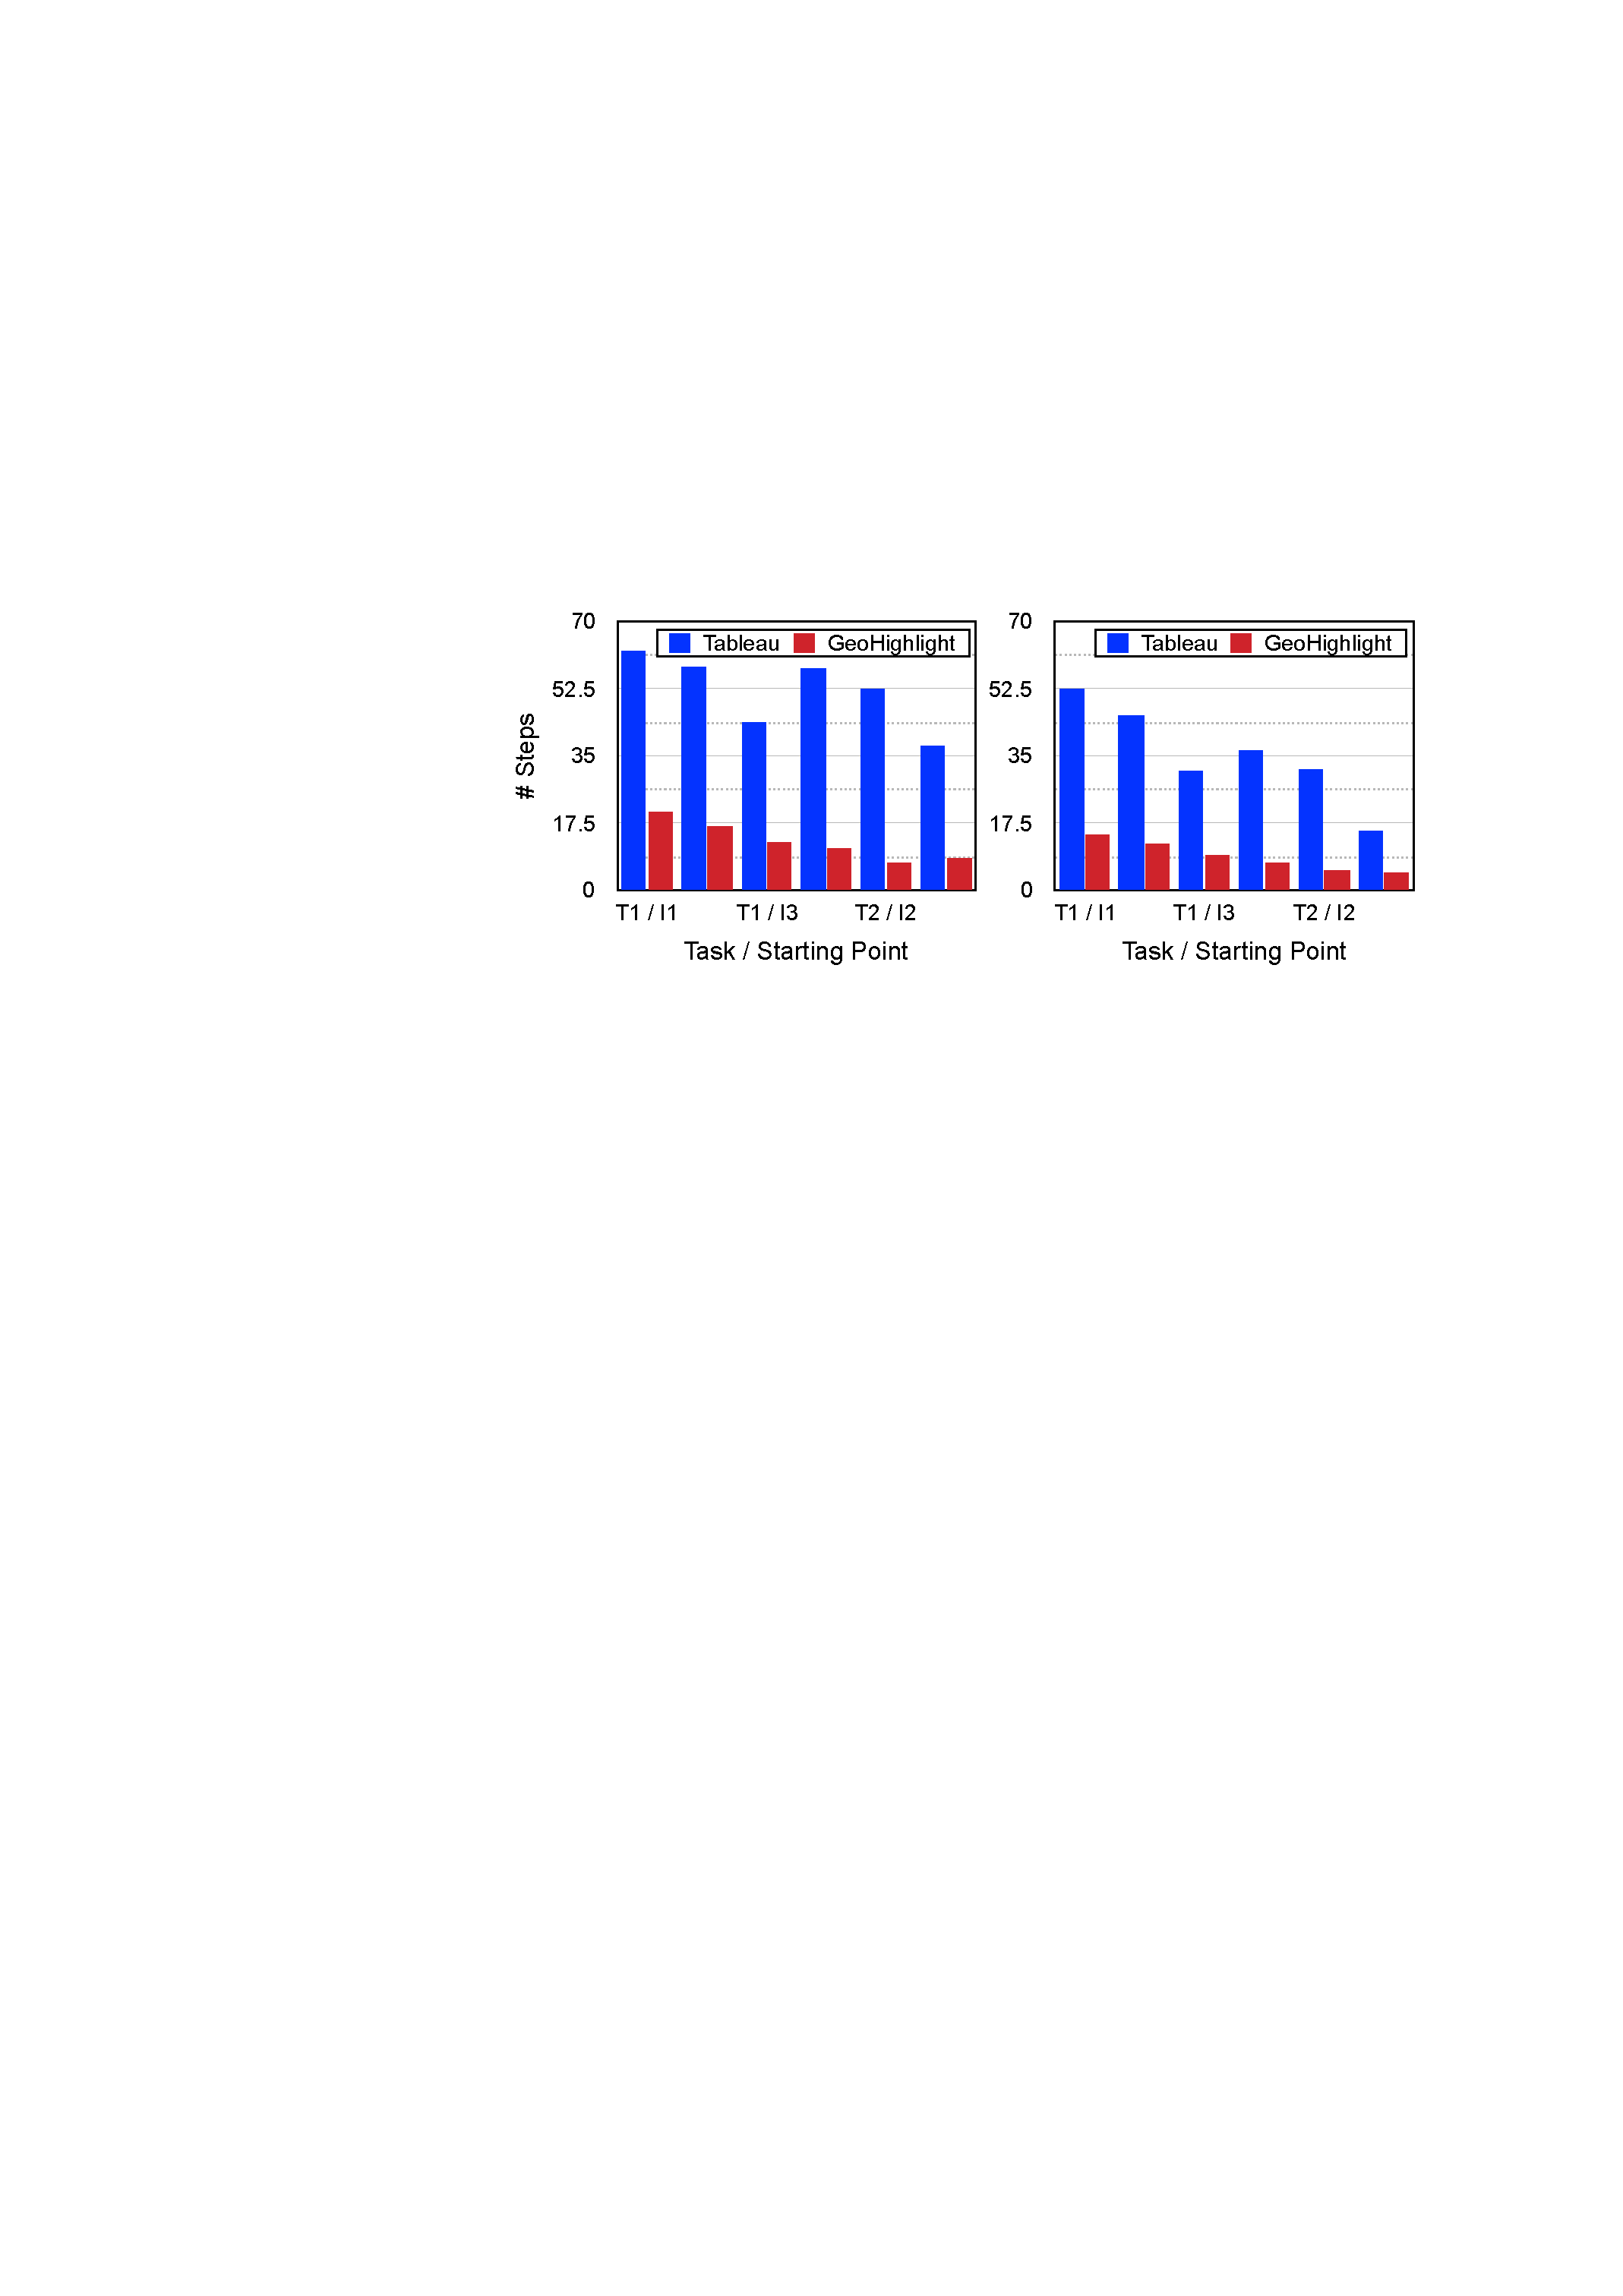
\includegraphics[width=\columnwidth]{figs/userstudy}
\caption{User Study}
\vspace{-5pt}
\label{fig:userstudy}
\end{figure}


% We also asked our participants about their insights on \framework. We ask them to rate the following metric on a 5-star scale: {\em usefulness} and {\em ease-of-use}. In summary, we found that \colorred{[explain received results]}.
% \section{Related Work}
\label{sec:rel}
The literature contains several instances of feedback exploitation to guide the analyst in further analysis steps (e.g., \cite{boley2013one}). The common approach is a top-$k$ processing methodology in order to prune the search space based on the explicit feedback and recommend a small subset of interesting results of size~$k$.  As the key challenge is unify
explicit and implicit feedback, some works~\cite{AoidhBW07,Ballatore2008,Liu:2010} propose models from both explicit and implicit feedback in order to capture user preferences. A clear distinction of \sgg\ is that it doesn't aim for pruning, but leveraging the actual data with potential interesting results that the analyst may miss due to the huge volume of spatial data. While in top-$k$ processing algorithms, analyst choices are limited to $k$, \sgg\ has a freedom of choice where highlights get seamlessly updated with new analyst choices. 

\vspace{2pt}
There exist few instances of information-highlighting methods in the literature \cite{Liang2010,Robinson2011,wongsuphasawat2016voyager,willett2007scented}. All these methods are {\em objective} and do not apply to the context of spatial guidance where user feedback is involved.  In terms of recommendation, few approaches focus on spatial dimension \cite{Bao2015,Levandoski:2012} while the context and result diversification are missing.

\vspace{2pt}
Considering approaches to better generate regions as polygons and verify is a point is inside a defined region, we analysed some works. These approaches use, in general, clustered points to create concave and convex polygons. \cite{Bevis1989} proposes an algorithm for determining if any given point P, on the surface of a sphere is located inside, outside, or along the border of an arbitrary spherical polygon. \cite{DUCKHAM2008} and  \cite{FADILI2004} propose algorithms for constructing a non-convex polygons that characterizes the shape of a set of input points in the plane. These solutions consider only the definition of shapes in their proposals. \cite{ARAMPATZIS2006} and \cite{Galton2006} propose solutions for delineation of imprecise regions, either convex or concave. The most efficient and adequate and appropriated solution for generation of  convex polygons to our solution was the Quickhull  algorithm~\cite{Barber:1996}.
% \newpage
\section{Conclusion}
\label{sec:conc}
We addressed the problem of generic guidance and introduced \framework, the first efficient interactive highlighting approach in spatiotemporal data. We formulated our problem in form of a constrained optimization and proposed {\sc Highlighter}, a greedy algorithm to highlight $k$-best points for a given point of interest within a time limit. We discussed genericness of our approach by materializing few examples from restaurant and taxi datasets. We also showed the efficiency and usability of our framework in form of performance experiments and user study. There are several directions of improvement for this work. Specifically, we want to consider an analyst profile vector which is built during interactive steps and will be exploited to return more analyst-tailored results.


\bibliographystyle{abbrv}
\bibliography{main} 

\end{document}
